\documentclass[aps,pra,onecolumn,superscriptaddress]{revtex4}

\pdfoutput=1

\usepackage[colorlinks=true,linkcolor=blue,citecolor=blue,urlcolor=blue]{hyperref}

\usepackage{hyperref}
%\usepackage{geometry}
\usepackage{setspace} %to set 1.5 spacing in text
\usepackage{graphicx}
\usepackage{subfigure}
%\usepackage[font=small,labelfont=bf]{caption}%to customize captions
%\usepackage{tikz} %to draw graphics
\usepackage{amsmath}
\usepackage{color}
\usepackage{amsmath}
\usepackage{amssymb}
\usepackage{verbatim}
\usepackage{latexsym}
\usepackage{enumerate} % to change the numbering of 'enumerate'
\usepackage{bm} % for bold face mathematical symbols


\bibliographystyle{apsrev4-1}


\setcounter{tocdepth}{3}

\begin{document}

\title{Supplemental Material for ``First principles study of the dynamic Jahn-Teller distortion of the neutral vacancy in diamond''}

\author{Joseph C.\ A.\ Prentice}
\affiliation{TCM Group, Cavendish Laboratory, University of Cambridge,
  J.\ J.\ Thomson Avenue, Cambridge CB3 0HE, United Kingdom}
\author{Bartomeu Monserrat}
\affiliation{TCM Group, Cavendish Laboratory, University of Cambridge,
  J.\ J.\ Thomson Avenue, Cambridge CB3 0HE, United Kingdom}
\affiliation{Department of Physics and Astronomy, Rutgers University,
  Piscataway, New Jersey 08854-8019, USA}
\author{R.\ J.\ Needs}
\affiliation{TCM Group, Cavendish Laboratory, University of Cambridge,
  J.\ J.\ Thomson Avenue, Cambridge CB3 0HE, United Kingdom}


\date{\today}

\maketitle

\section{Pseudopotentials}

All density functional theory calculations were performed using {\sc CASTEP} version $7.0.3$, and its own ``on-the-fly'' ultrasoft pseudopotential for carbon. The definition string for the pseudopotential was:

\begin{verbatim}
2|1.4|1.4|1.3|6|10|12|20:21(qc=6)
\end{verbatim}

\section{Equilibrium positions}

The equilibrium positions of the 255 atoms in the tetrahedral symmetry structure with the experimental lattice constant are given in the file \texttt{TdSymmetry.cif}. The 4 nearest neighbours of the vacancy are the 1st, 37th, 41st and 69th atoms listed.

\section{Soft mode displacement patterns}

The displacement patterns of the two soft modes, labelled by $u_1$ and $u_2$ in the main text, are given in the files \texttt{u1Displacements.cif} and \texttt{u2Displacements.cif}. The 4 nearest neighbours of the vacancy are the 1st, 37th, 41st and 69th atoms listed. 

\section{Born-Oppenheimer energy surface slices}

Figure \ref{fig:CrossSections} shows two cross-sections of the BO surface in the plane spanned by the two soft modes of the tetrahedral structure. Figure \ref{subfig:mintomax} shows a slice running from one of the three minima of the surface to the opposite high point passing through the origin of coordinates $(u_1,u_2)=(0,0)$. Figure \ref{subfig:mintomin} shows a slice that runs from one minimum to an adjacent minimum, and this line does not cross the origin of coordinates. 

\begin{figure}
\begin{center}
\subfigure[][]{
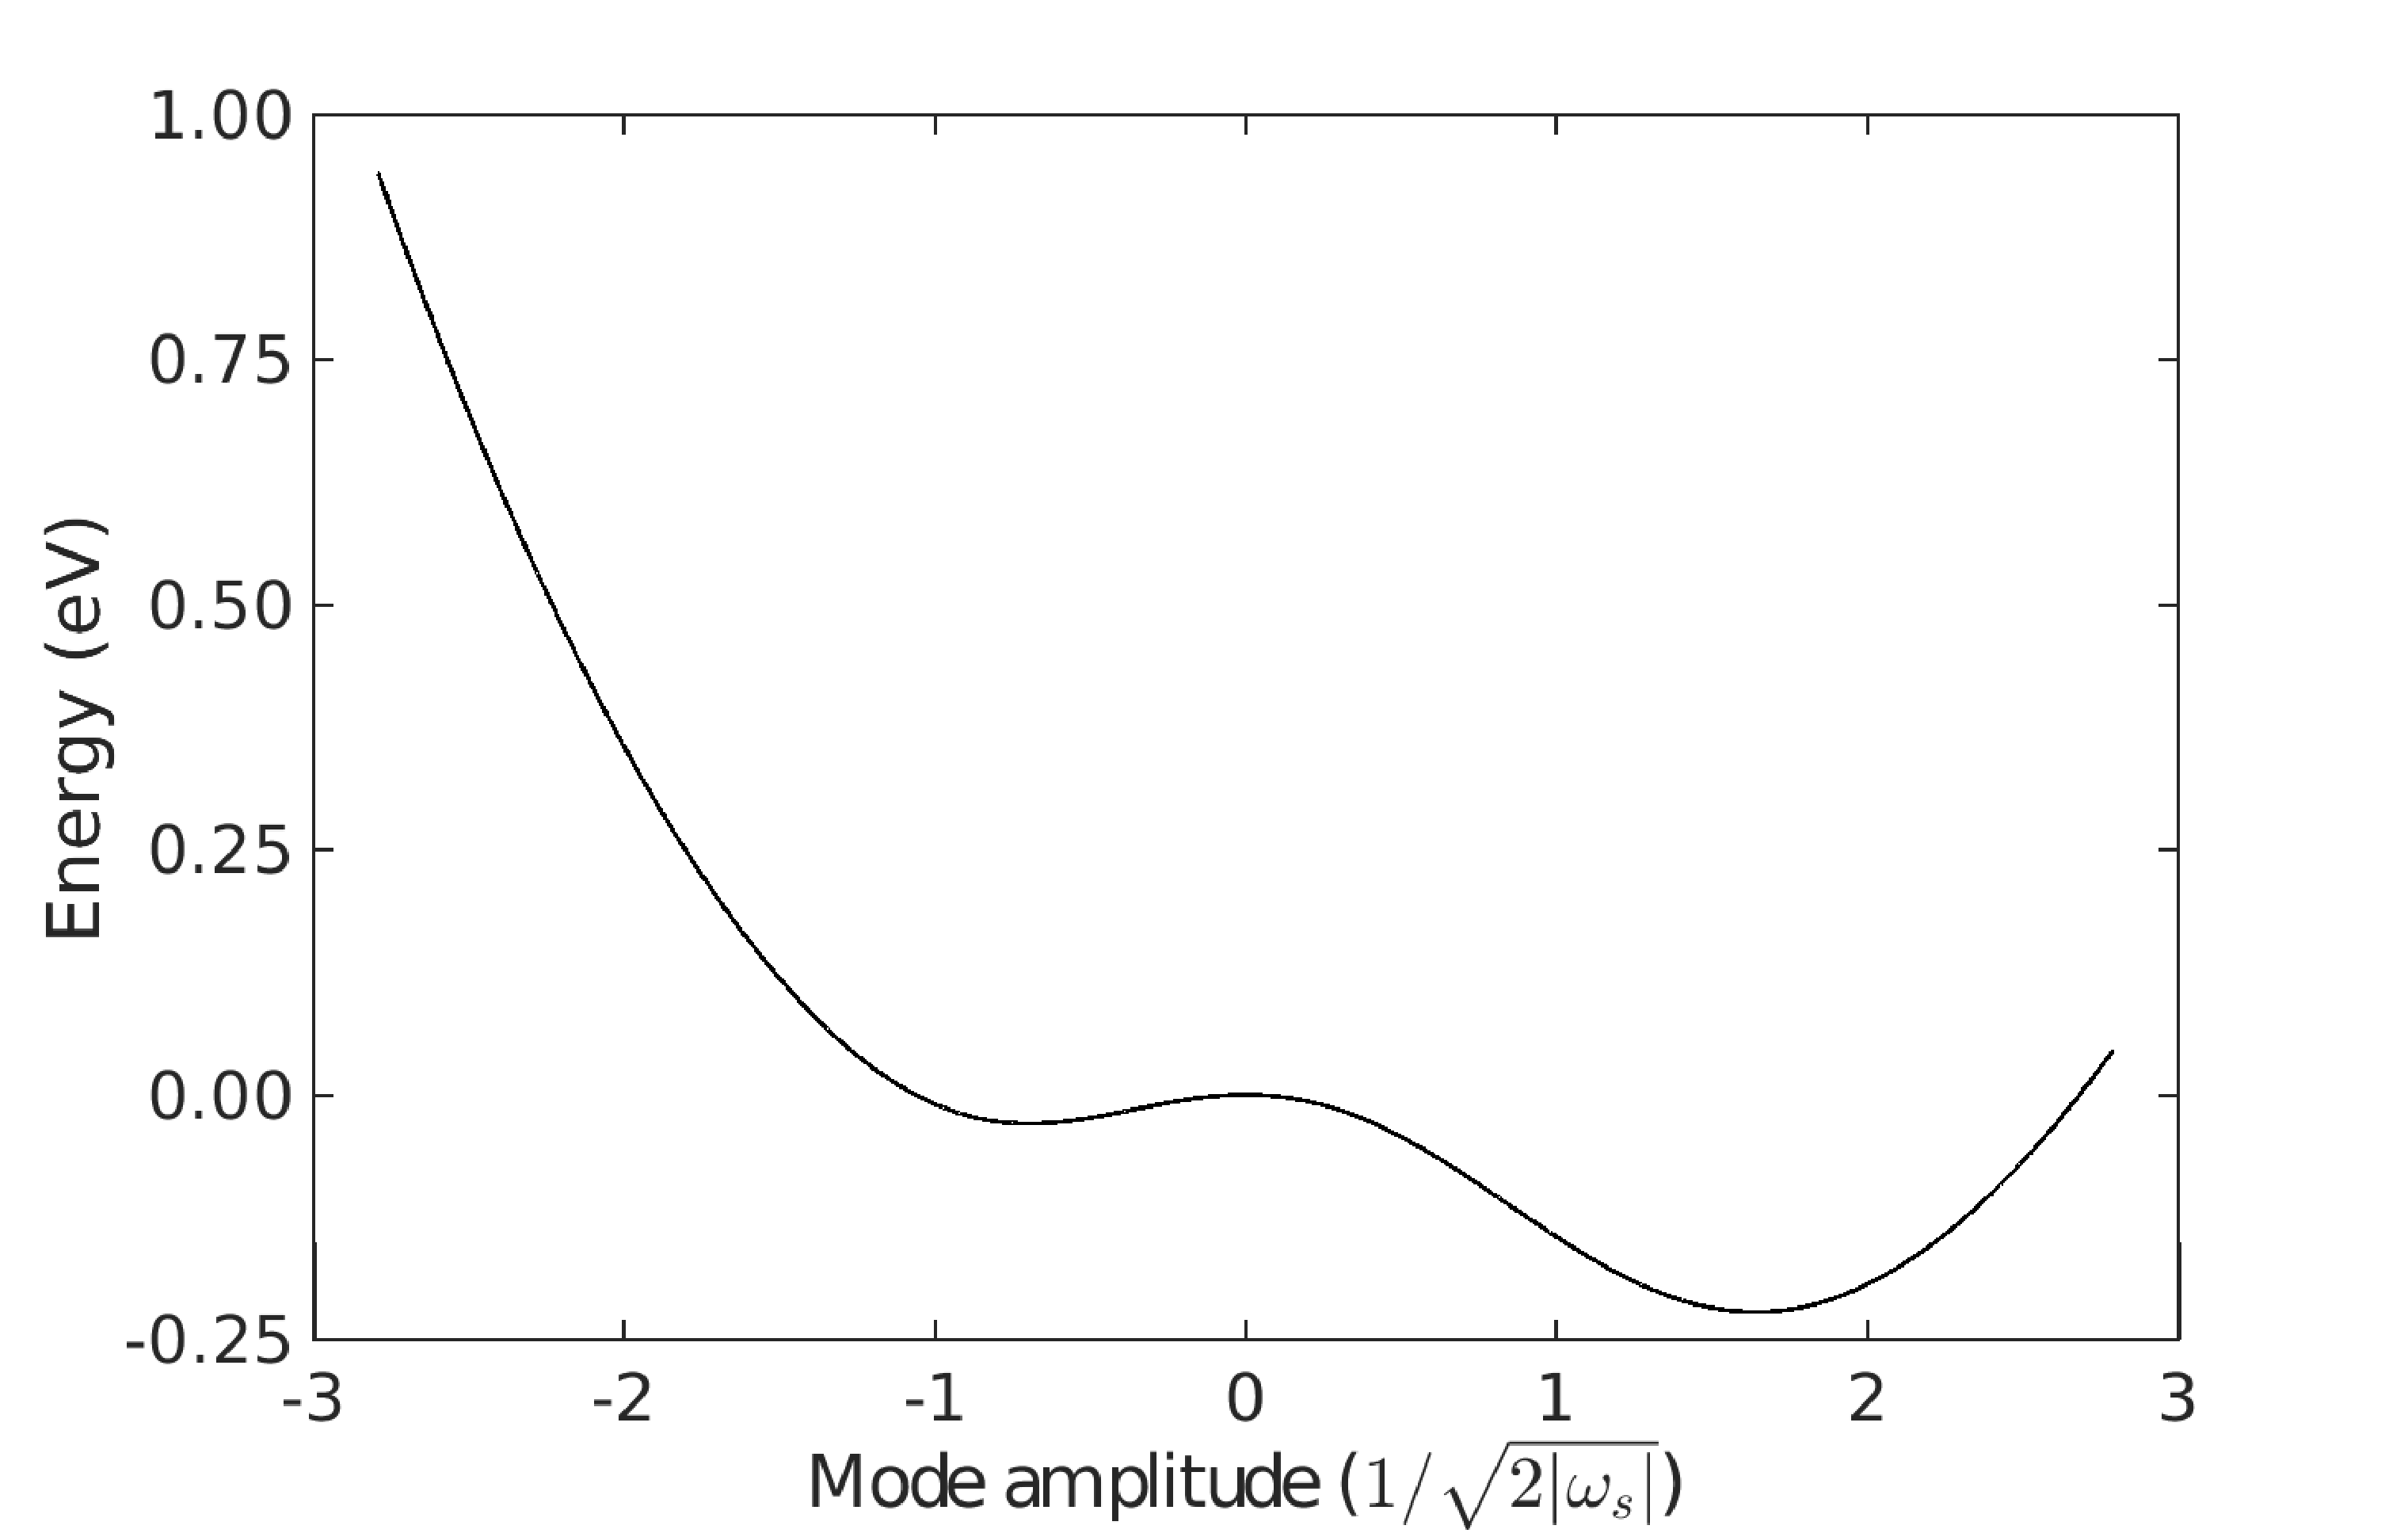
\includegraphics[width=0.75\textwidth]{MinToMax.eps}
\label{subfig:mintomax}
}
~
\subfigure[][]{
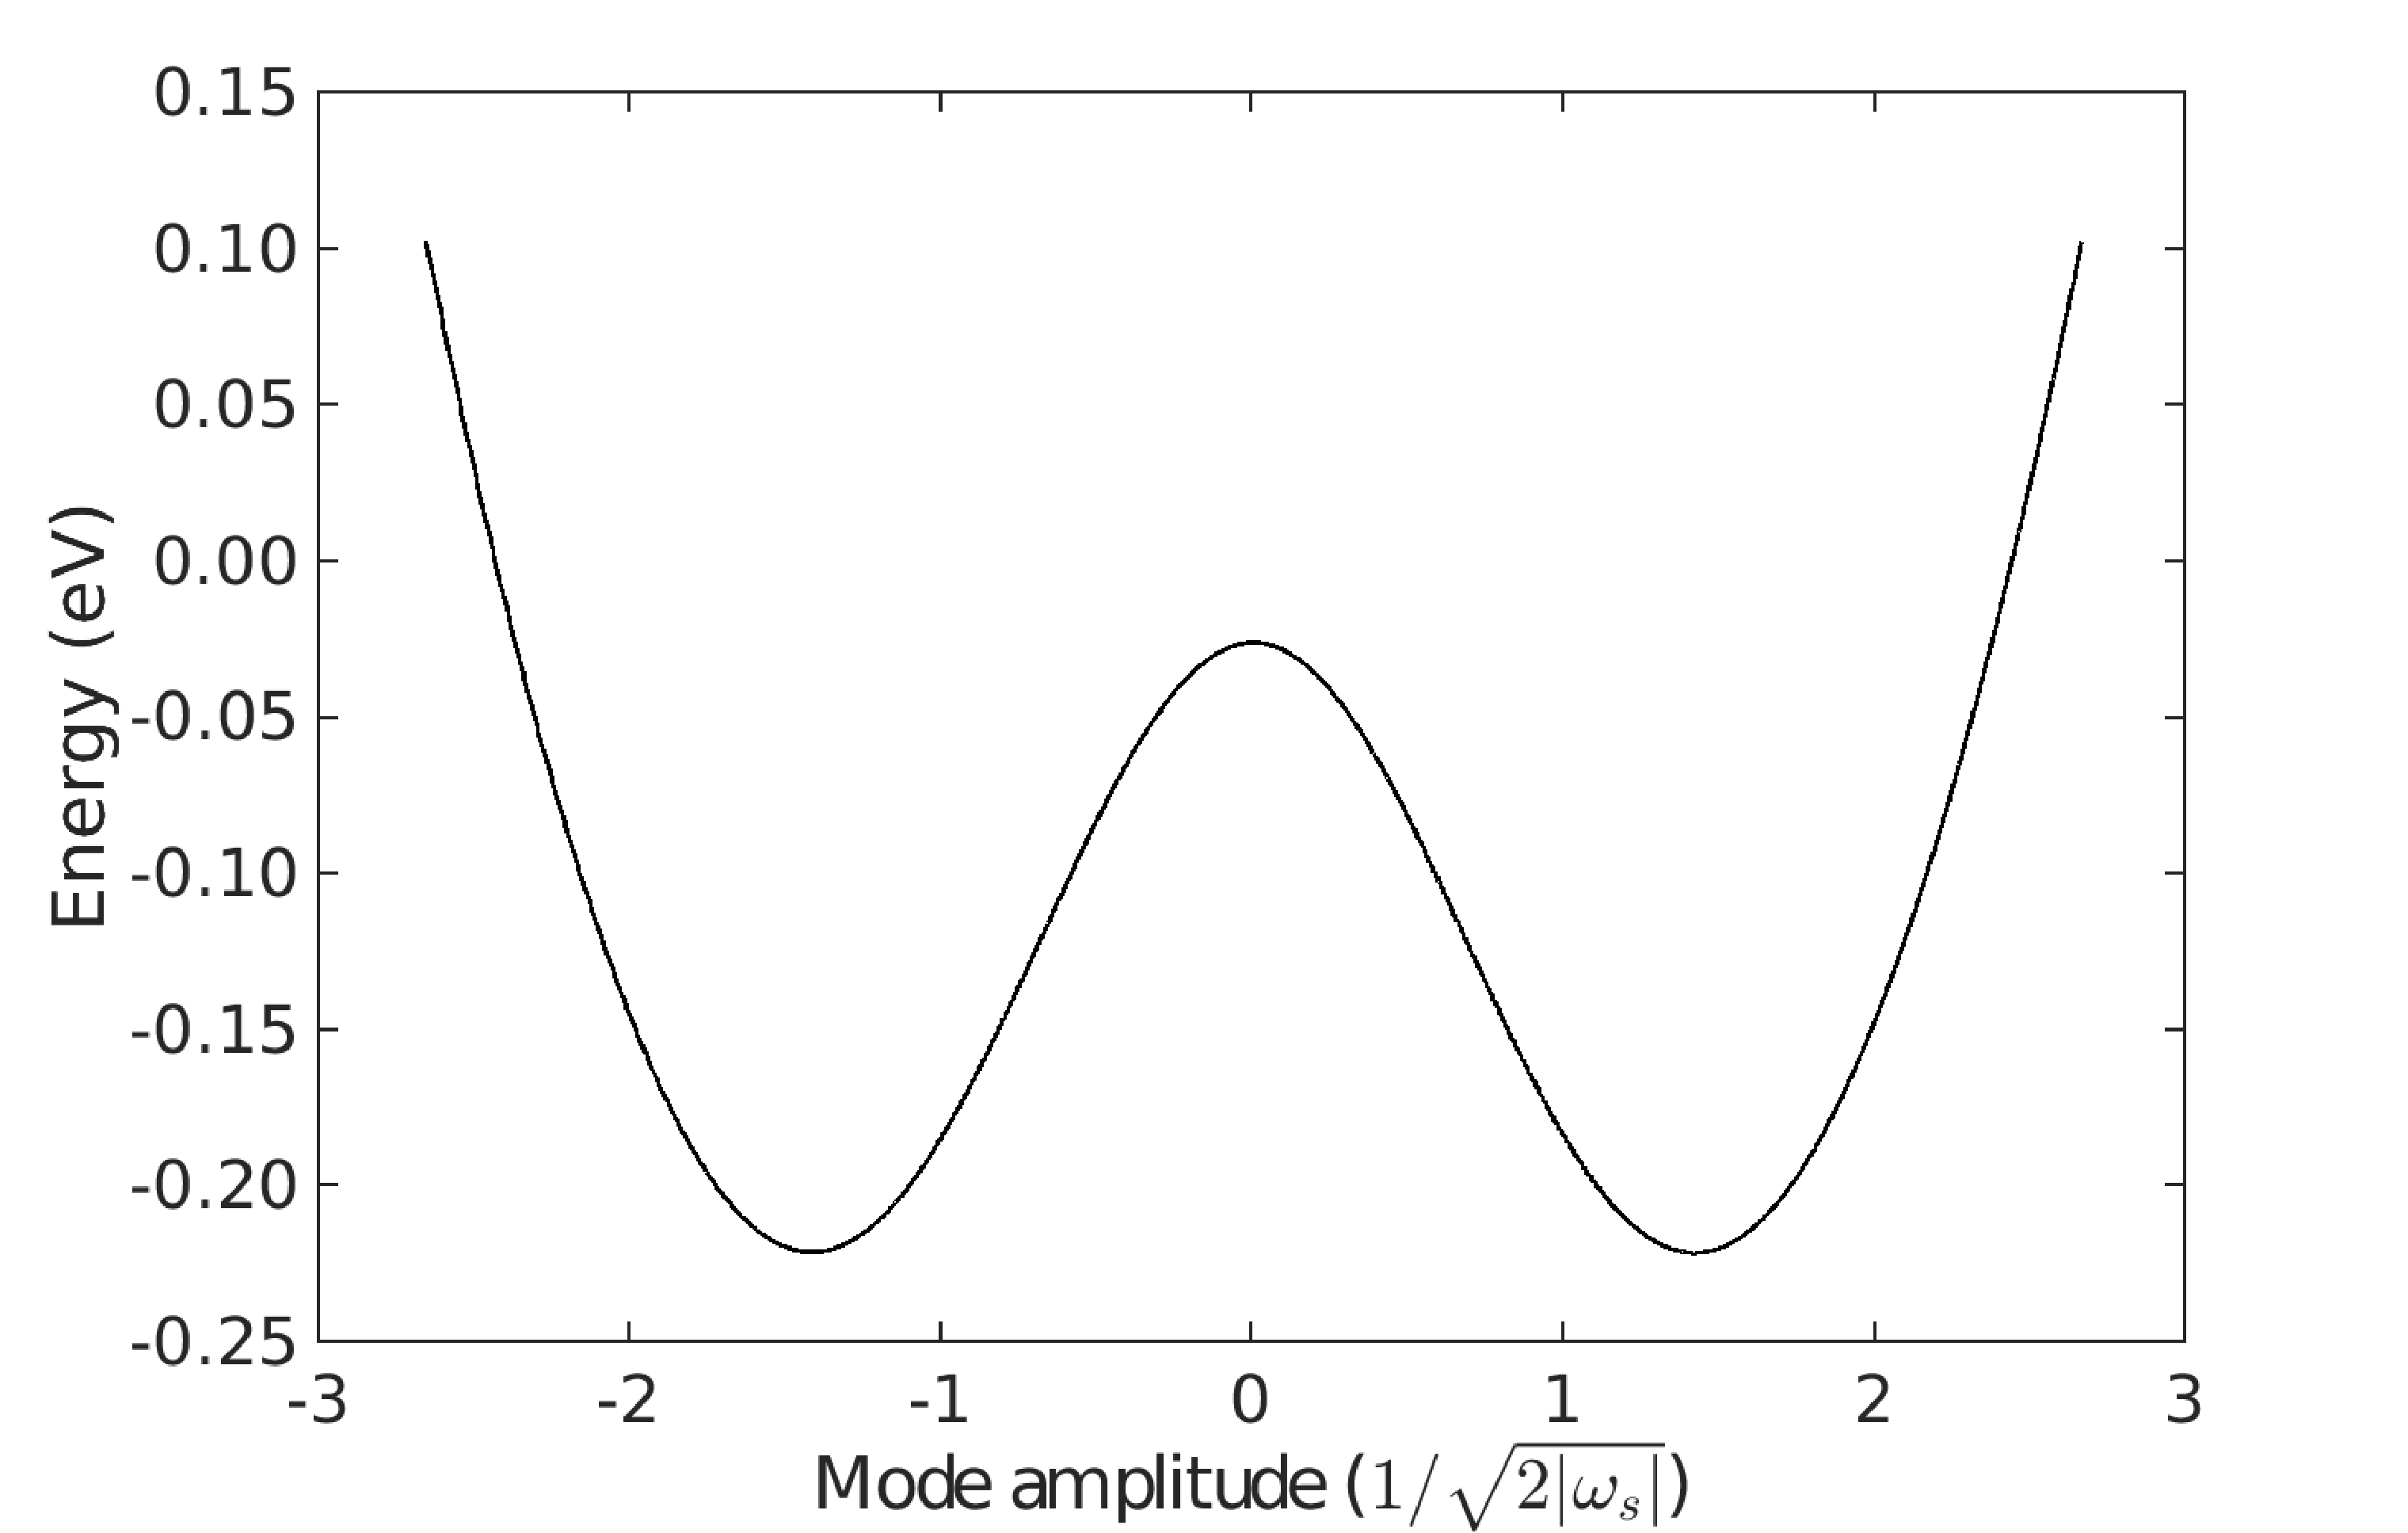
\includegraphics[width=0.75\textwidth]{MinToMin.eps}
\label{subfig:mintomin}
}
\end{center}
\caption{Slices through the BO surface in the plane spanned by the two soft modes of the tetrahedral structure. The slice in (a) runs through one minimum and the origin, also passing through the high point of the graph opposite. The slice in (b) runs through two adjacent minima. In (b), the point midway between the two minima is taken as the zero point of the mode amplitude.} \label{fig:CrossSections}
\end{figure}

\end{document}
